\chapter{Resultados e Discussão}\label{cap:resultados}

\section{Desafio em trajeto especifíco fácil}

O primeiro e único treino foi executado como agente percorrendo somente um percurso em linha reta, conforme a imagem abaixo.

\begin{figure}[h]
    \centering
    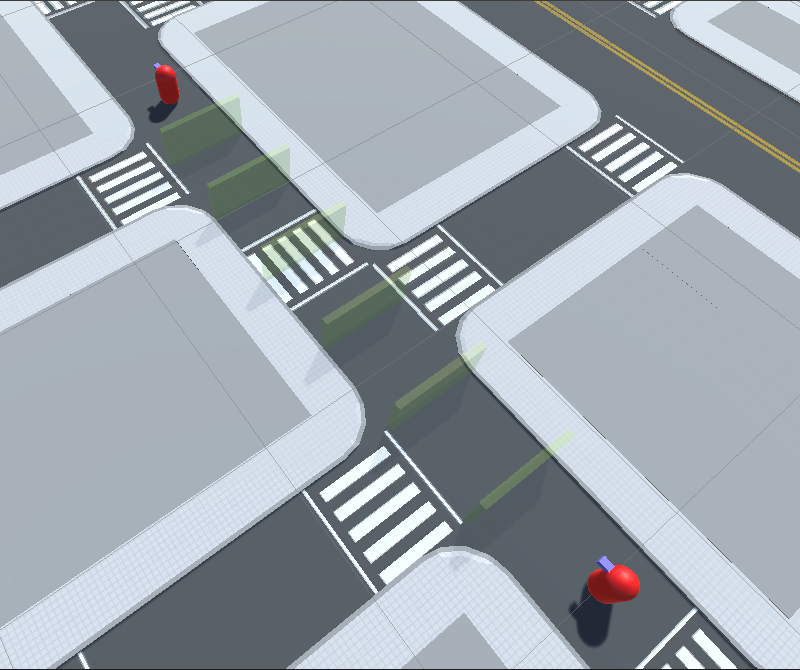
\includegraphics[scale=0.25]{figs/rotas/path_14.png}
     \caption{O percurso executado no primeiro treino. A cápsula vermelha no canto inferior direito indica a posição inicial do veículo e a na parte superior esquerdo indica o destino.}
     \label{fig:rota-1}
\end{figure}
 
\begin{figure}[h]
    \centering
    \includegraphics[scale=0.35]{figs/treinos/treino-1/política.png}
     \caption{Estatísticas referentes a política. O primeiro gráfico é a entropia, decaindo como é esperado. O terceiro gráfico é o Extrinsic Value estimate, sobe e estabiliza, conforme esperado}
     \label{fig:treino-1-politica}
\end{figure}

\begin{figure}[h]
    \centering
    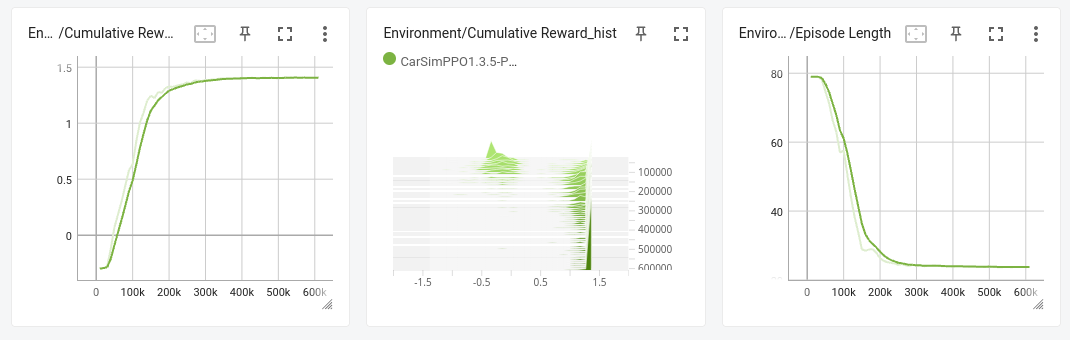
\includegraphics[scale=0.35]{figs/treinos/treino-1/ambiente.png}
     \caption{Estatísticas do ambiente. O primeiro gráfico é o acumulado de recompensa, o segundo é um histograma das distribuições de recompens. O terceiro é a duração do episódio.}
     \label{fig:treino-1-ambiente}
\end{figure}

\subsection*{Análise}
O treino foi bem sucedido, o agente soube conduzir bem o veículo. Vendo o gráfico 1 da figura 9, pode-se notar o crescimento exponencial da recompensa e então sua estabilização quando atinge o máximo da recompensa que é possível receber. Também percebe-se que na mesma velocidade mas desta vez em sentido descendente a duração média do episódio, rapidamente cai pois o agente já dominou o trajeto. Isso é o suficiente para este trajeto, podemos treinar o agente em um novo desafio especifíco mas com um trajeto mais complexo.


\section{Desafio em trajeto específico dificuldade média}
Aqui o treino foi feito em dois trajetos (identificados por Path(8) e Path(0) no projeto), ambos exigem que o agente faça uma conversão do veículo.

Neste desafio foi necessário uma melhoria no agente, foi aumentado o número de sensores, agora ele possui dois \textit{components} Ray Perception Sensor 3D, o primeiro é para visão frontal e detecta os checkpoints e obstáculos e o segundo é uma visão para todas as direções do carro servindo para detecção apenas de obstáculos. Isso foi necessário pois na primeira versão havia pontos cegos, durante os testes o veículo não completava pois os sensores não detectavam o destino em sua frente.


\begin{figure}[h]
    \centering
    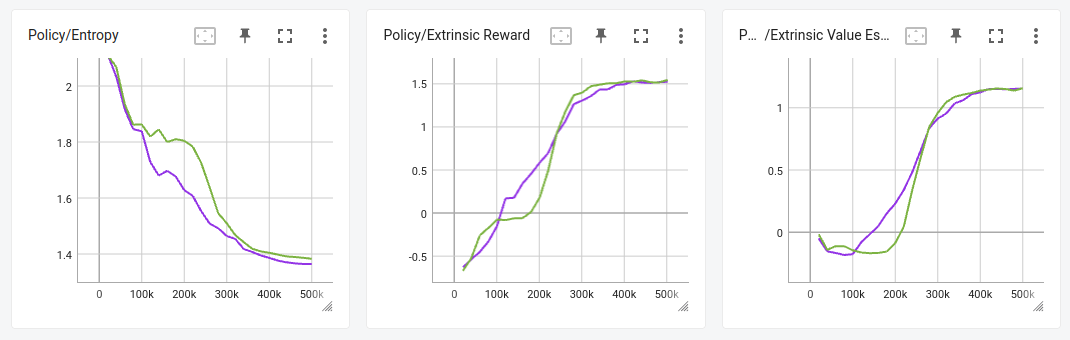
\includegraphics[scale=0.35]{figs/treinos/desafio-mediano/politica.png}
    \caption{Estatísticas referentes a política do segundo desafio nas duas rotas, em verde a rota \textit{Path(8)} e em roxo a rota \textit{Path(0)}.}
\end{figure}

\begin{figure}[h]
    \centering
    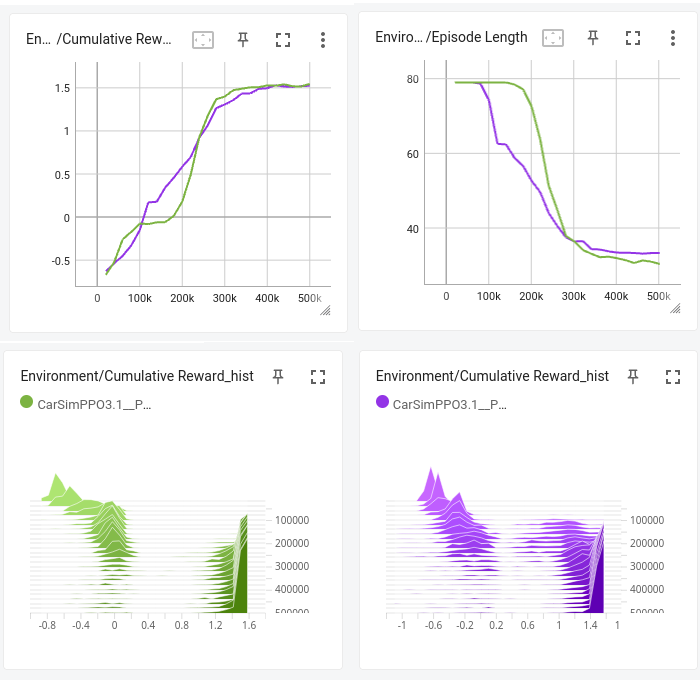
\includegraphics[scale=1.5]{figs/treinos/desafio-mediano/ambiente-2por2.png}
    \caption{Estatísticas do ambiente do segundo desafio para ambas as rotas. Em cima os gráficos de recompensa e duração do episódio, abaixo os histogramas.}
\end{figure}


\subsection*{Análise}
O treinamento não encontrou problemas para convergir neste desafio, para ambas as rotas foram dados 500 mil passos de treino mas por volta de 400 mil passos a recompensa mediana se estabilizou no topo mostrando que o modelo convergiu. De acordo com os histrogramas o agente conclui praticamente todos os episódios e isso se reflete nos testes onde o agente chega ao destino em todos as tentativas, subindo a calçada somente uma única vez.

\section{Desafio em trajeto específico difícil}
Para este desafio foi testado em três rotas diferentes, duas delas possui duas curvas e a terceira possui três curvas.

\begin{figure}[h]
    \centering
    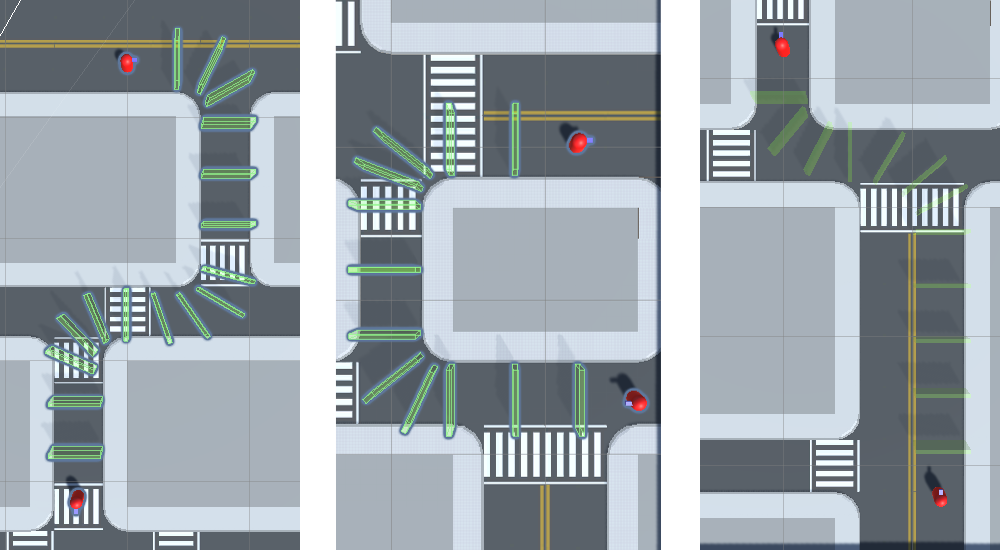
\includegraphics{figs/treinos/desafio-dificil/rotas.png}
    \caption{As três rotas difíceis envolve mais de uma curva, a esquerda o path(3) que possui três curvas sendo o mais complexo dos trajetos. Os outros dois são o path(5) e path(6) que possuem 2 curvas cada.}
\end{figure}

\begin{figure}[h]
    \centering
    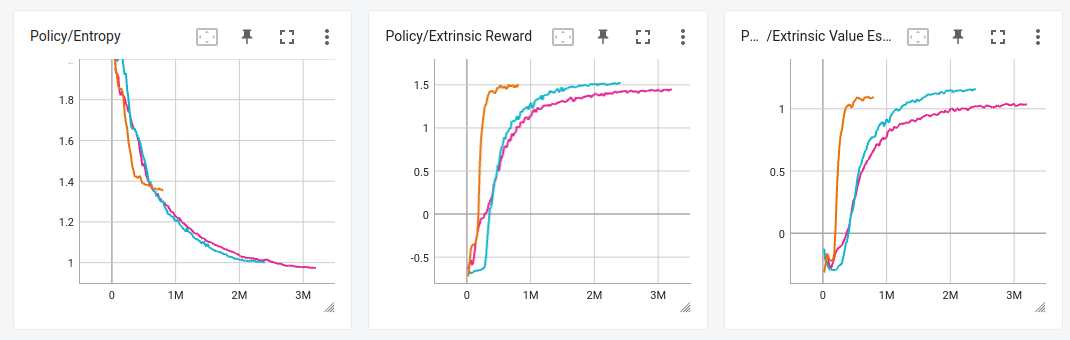
\includegraphics[scale=0.35]{figs/treinos/desafio-dificil/politica.png}
    \caption{Estatísticas referentes a política do desafio em rotas difíceis. \textit{Path(3)}, \textit{Path(5)} e \textit{Path(6)} em laranja, azul e magenta, respectivamente.}
\end{figure}

\begin{figure}[h]
    \centering
    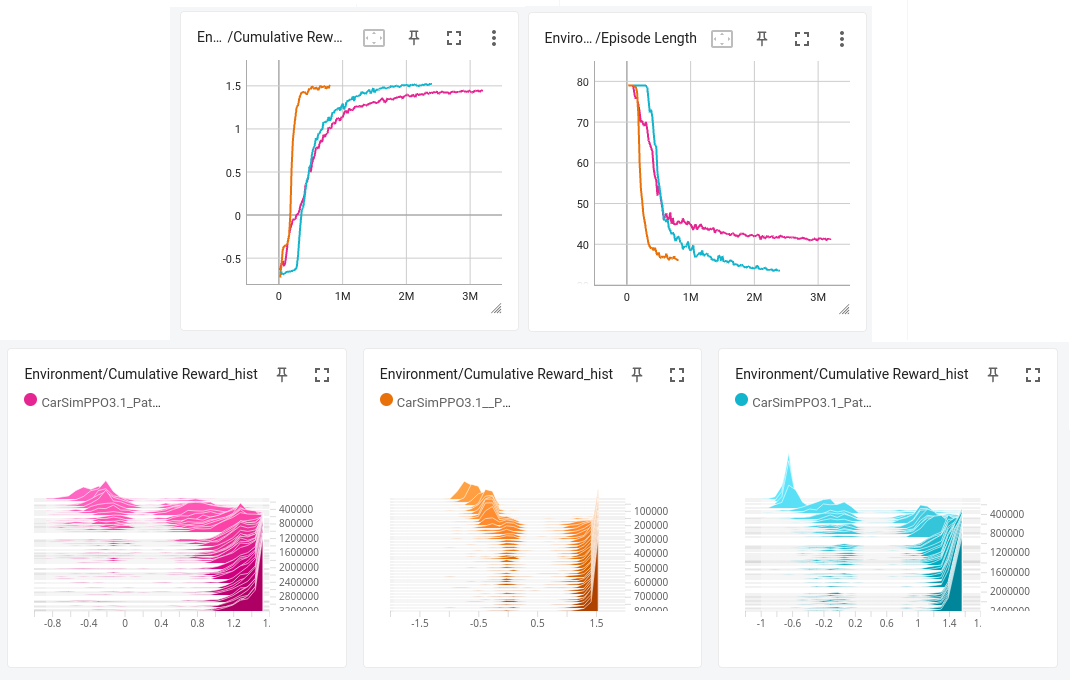
\includegraphics[scale=1.25]{figs/treinos/desafio-dificil/ambiente-completo.png}
    \caption{Estatísticas referentes ao ambiente do desafio em rotas difíceis. Em cima os gráficos da recompensa e duração dos episódios, abaixo os histrogramas de recompensa.}
\end{figure}

\subsection*{Análise}
Neste desafio ficou claro que o agente teve muito mais dificuldade de convergir para ter um desempenho ótimo. Embora os três trajetos estejam no mesmo grupo de desafio cada uma das três rotas exigiu uma quantidade de steps maior para covergir, o \textit{Path(5)}, que envolvia fazer duas curvas a direita, foi o mais fácil para o agente, o treino durou 800 mil passos mas por volta de 500 mil steps já havia atingido a média máxima de recompensa. Porém, as rotas Path(3) e Path(6) demoraram respectivamente 3,2 milhões e 2,4 milhões de steps para atingir o mesmo nível, sendo que ao final do treino o primeiro ainda ficou com uma recompensa média ligeiramente abaixo dos demais.
\section{Desafio em todos os trajetos}

\begin{figure}[h]
    \centering
    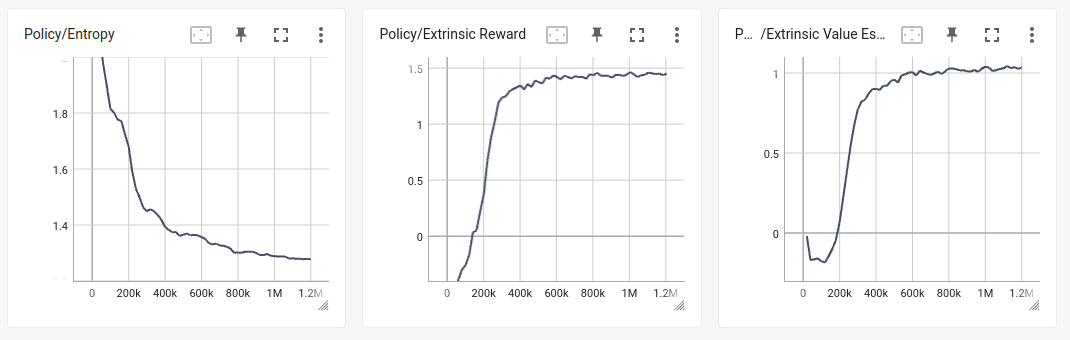
\includegraphics[scale=0.35]{figs/treinos/desafio-geral/politica.png}
    \caption{Estatísticas referentes a política do desafio geral.}
\end{figure}

\begin{figure}[h]
    \centering
    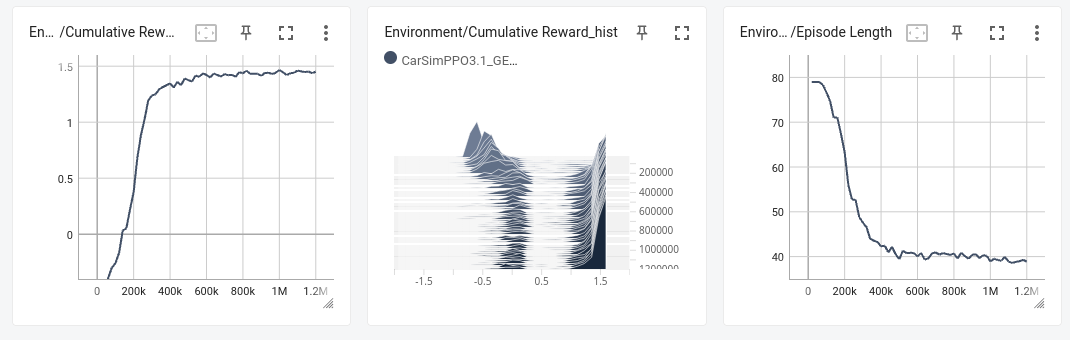
\includegraphics[scale=0.35]{figs/treinos/desafio-geral/ambiente.png}
    \caption{Estatísticas do ambiente do desafio geral.}
\end{figure}

\begin{table}[htpb]
    \centering
    \caption{Consolidado do teste geral, inclui todas tentativas e suas recompensas e a recompensa média por rota.}
    \label{resultado-tabela-geral}
    \begin{tabular}{|l|c|c|c|c|c|c|r|}
         \hline
         \small{Rota} & \small{C. T. 1} & \small{Rec. 1}  & \small{C. T. 2} &\small{Rec. 2} & \small{C. T. 3} &\small{Rec. 3} &\small{Rec. média}   \\ \hline
            Path(0)   &      sim        &   1             &    sim          &      1        &    sim          &      1     &      1                 \\ \hline
            Path(1)   &      sim        &   1             &    sim          &      1        &    sim          &      1     &      1                 \\ \hline
            Path(2)   &      sim        &   1             &    sim          &      1        &    sim          &      1     &      1                 \\ \hline
            Path(3)   &      não        &   -0.18         &    sim          &      0.85     &    sim          &      1     &      0.56              \\ \hline
            Path(4)   &      sim        &   1             &    sim          &      1        &    sim          &      1     &      1                 \\ \hline
            Path(5)   &      sim        &   1             &    sim          &      0.8      &    sim          &      1     &      0.93              \\ \hline
            Path(6)   &      sim        &   1             &    não          &      -0.31    &    sim          &      1     &      0.56              \\ \hline
            Path(7)   &      sim        &   0.85          &    sim          &      1        &    sim          &      0.9   &      0.91              \\ \hline
            Path(8)   &      sim        &   1             &    sim          &      0.9      &    sim          &      1     &      0.96              \\ \hline
            Path(9)   &      sim        &   1             &    sim          &      0.95     &    sim          &      1     &      0.98              \\ \hline
            Path(10)  &      não        &   0.12          &    não          &      0.02     &    sim          &      1     &      0.38              \\ \hline
            Path(11)  &      sim        &   1             &    sim          &      1        &    sim          &      1     &      1                 \\ \hline
            Path(12)  &      sim        &   1             &    sim          &      1        &    sim          &      1     &      1                 \\ \hline
            Path(13)  &      sim        &   1             &    sim          &      1        &    sim          &      1     &      1                 \\ \hline
            Path(14)  &      sim        &   1             &    sim          &      1        &    sim          &      1     &      1                 \\ \hline
            Path(15)  &      sim        &   1             &    sim          &      1        &    sim          &      1     &      1                 \\ \hline
            Path(16)  &      sim        &   1             &    sim          &      1        &    sim          &      1     &      1                 \\ \hline
    \end{tabular}
\end{table}
\subsection*{Análise}
O desafio foi um sucesso, o treino utilizando de PPO convergiu por volta dos 600 mil passos, metade do limite, o agente "percebeu" rapidamente que seu objetivo era atingir cada checkpoint até o destino. O teste no geral foi positivo sendo perfeito em 10 dos 17 trajetos, obtendo 0,89 de média geral e concluindo 48 dos 51 tentativas. 
Porém se fizermos um recorte de trajetos difíceis (duas ou mais curvas) teremos um resultado não tão satisfatório. Neste caso seriam além dos envolvidos no desafio anterior, seriam os Path's de número 7, 10, 12 e 14, teríamos 18 conclusões de 21 corridas feitas (85\%), todas as vezes que o agente falhou foram em um desses e com média de apenas 0,63 de recompensa.